\documentclass[11pt]{article}

\usepackage[a4paper,margin=2.2cm]{geometry}
\usepackage{amsmath,amssymb}
\usepackage{graphicx}
\usepackage{subcaption}
\usepackage{booktabs}
\usepackage{siunitx}
\usepackage{xcolor}
\usepackage{listings}
\usepackage{tikz}
\usetikzlibrary{patterns}
\usepackage[hidelinks]{hyperref}
\usepackage{caption}
\captionsetup{font=small}

% ---- shorthands ----
\newcommand{\eox}{\varepsilon_{\mathrm{ox}}}
\newcommand{\esi}{\varepsilon_{\mathrm{si}}}
\newcommand{\epso}{\varepsilon_{0}}
\newcommand{\tox}{t_{\mathrm{ox}}}
\newcommand{\tsi}{t_{\mathrm{si}}}
\newcommand{\Heff}{H_{\mathrm{eff}}}
\newcommand{\Lx}{L_{x}}
\newcommand{\phih}{\phi_{h}}
\newcommand{\phip}{\phi_{p}}
\newcommand{\dd}{\mathrm{d}}
\newcommand{\ii}{\mathrm{i}}

\lstset{basicstyle=\ttfamily\footnotesize,breaklines=true,frame=single,
        columns=fullflexible,keepspaces=true,xleftmargin=4pt,framexleftmargin=4pt}

\title{\vspace{-1.2cm}\textbf{The Fig.~4 Potential Distribution of Nakagawa 1990,
Solved Four Ways}\\[4pt]
\large Finite Volumes, Conformal Mapping and a Green's Function for a
Thin-SOI High-Voltage Device\\
\normalsize Structure~B, \SI{500}{\volt} --- theory, algorithm, formulae and plots}
\author{Independent reproduction workspace}
\date{}

\begin{document}
\maketitle
\vspace{-0.7cm}

\begin{abstract}
\noindent Figure~4 of Nakagawa \emph{et al.} (ISPSD~1990) shows that when a thin
(\SI{20}{\micro\meter}) silicon film on a buried oxide (BOX) fully depletes, more
than half of the applied \SI{500}{\volt} is forced across the thin oxide. This
report reproduces that two-dimensional potential map by \emph{four independent
methods} and cross-validates them: (i)~a $1$-D vertical model, (ii)~a
finite-volume Poisson solve, (iii)~an analytic \emph{conformal map}
(Schwarz--Christoffel, Jacobi elliptic functions), and (iv)~an analytic
\emph{Green's function} (rectangle eigenfunction series). For each analytic method
we give the full derivation, the governing formulae, the algorithm, and the
generated plot. The two analytic methods agree to \SI{0.09}{\volt} RMS
($0.02\%$ of $V$) --- both predict an oxide voltage share of $\approx 58\%$ ---
and both track the finite-volume solve ($54\%$) to within the boundary-condition
idealisation they share. The charge-free limit is shown to give only $\approx
31\%$, isolating the donor space charge as the origin of the ``more than half''
result.
\end{abstract}

\tableofcontents
\medskip
\hrule

% ==========================================================================
\section{Device, physics and governing equations}
% ==========================================================================

\subsection{The structure}
Structure~B is a lateral cross-section (Fig.~\ref{fig:geom}): a silicon drift film
of thickness $\tsi=\SI{20}{\micro\meter}$ sits on a buried oxide of thickness
$\tox=\SI{3}{\micro\meter}$ over a grounded substrate. A drain electrode ($\phi=V$)
and a source electrode ($\phi=0$) occupy the top surface; a $p^{+}$ sinker grounds
the right silicon edge. A shallow $N$ donor sheet (dose $S_{D}=\SI{1.5e12}{\per\cm\squared}$
over the bottom $w_{n}=\SI{2}{\micro\meter}$ of the film, atop a background
$N_{D0}=\SI{1e14}{\per\cm\cubed}$) depletes and shields the bulk silicon. All
lengths are quoted in \si{\micro\meter}; the code works in CGS-practical units
(cm, V, \si{\per\cm\cubed}).

\begin{figure}[h]\centering
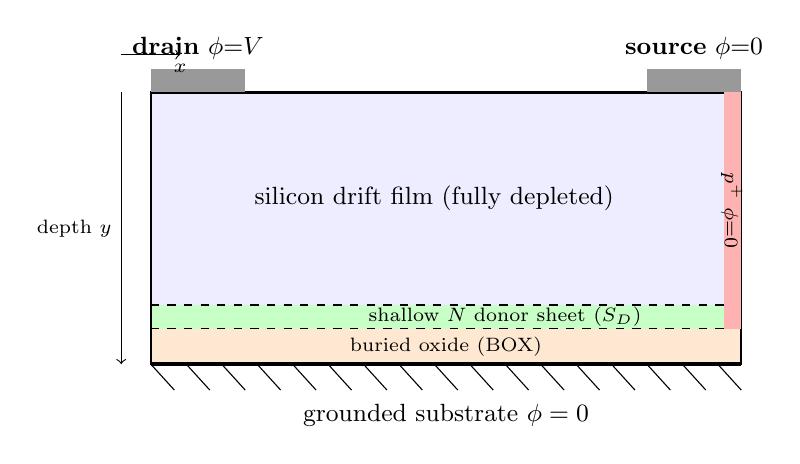
\begin{tikzpicture}[x=0.15cm,y=-0.15cm,font=\small]
  % --- layers (y increases downward) ---
  \fill[blue!7]   (0,0)  rectangle (50,18);   % silicon drift
  \fill[green!22] (0,18) rectangle (50,20);   % shallow donor sheet
  \fill[orange!18](0,20) rectangle (50,23);   % buried oxide
  % --- outlines ---
  \draw[thick] (0,0) rectangle (50,23);
  \draw[dashed] (0,20)--(50,20);
  \draw[dashed] (0,18)--(50,18);
  % --- electrodes ---
  \fill[gray!80] (0,-2) rectangle (8,0);
  \fill[gray!80] (42,-2) rectangle (50,0);
  \node[above] at (4,-2) {\textbf{drain} $\phi{=}V$};
  \node[above] at (46,-2) {\textbf{source} $\phi{=}0$};
  % --- p+ sinker (right Si edge) ---
  \fill[red!30] (48.5,0) rectangle (50,20);
  \node[rotate=-90] at (49.2,10) {\scriptsize $p^{+}\ \phi{=}0$};
  % --- substrate ground ---
  \draw[very thick] (0,23)--(50,23);
  \foreach \i in {0,3,...,48}{\draw (\i,23)--(\i+2,25.2);}
  \node[below] at (25,25.6) {grounded substrate $\phi=0$};
  % --- region labels ---
  \node at (24,9)  {silicon drift film (fully depleted)};
  \node at (30,19) {\scriptsize shallow $N$ donor sheet ($S_{D}$)};
  \node at (25,21.5){\scriptsize buried oxide (BOX)};
  % --- depth axis (lateral x is obvious; kept clear of electrodes/labels) ---
  \draw[->] (-2.5,0)--(-2.5,23) node[left,midway]{\scriptsize depth $y$};
  \draw[->] (-2.5,-3.2)--(2.5,-3.2) node[below]{\scriptsize $x$};
\end{tikzpicture}
\caption{Structure~B cross-section (not to scale). The fully-depleted silicon film
sits on the buried oxide over a grounded substrate; the shallow donor sheet shields
the bulk silicon, and the $p^{+}$ sinker grounds the right edge.}
\label{fig:geom}
\end{figure}

\begin{table}[h]\centering\small
\caption{Model parameters (identical across all four methods).}
\begin{tabular}{@{}llll@{}}
\toprule
$\tsi$ & \SI{20}{\micro\meter} & drain / source width & \SI{8}{\micro\meter} \\
$\tox$ & \SI{3}{\micro\meter}  & $w_{n}$ (donor sheet) & \SI{2}{\micro\meter} \\
$\Lx$  & \SI{50}{\micro\meter} & $N_{D0}$ & \SI{1e14}{\per\cm\cubed} \\
$V$    & \SI{500}{\volt}       & $S_{D}$  & \SI{1.5e12}{\per\cm\squared} \\
$\esi=11.7\,\epso$ & $\eox=3.9\,\epso$ & $q=\SI{1.602e-19}{\coulomb}$ & $\epso=\SI{8.854e-14}{\farad\per\cm}$\\
\bottomrule
\end{tabular}
\end{table}

\subsection{Poisson's equation with two dielectrics}
With $x$ lateral and $y$ the depth (downward), the electrostatic potential
$\phi(x,y)$ obeys
\begin{equation}
\nabla\!\cdot\!\big(\varepsilon(x,y)\,\nabla\phi\big) = -\rho(x,y),
\qquad
\rho = q\,N(y)\ \text{in Si},\quad \rho=0\ \text{in oxide},
\label{eq:poisson}
\end{equation}
with $\varepsilon=\esi$ in the silicon ($0\le y<\tsi$) and $\varepsilon=\eox$ in
the oxide ($\tsi\le y<H$), $H=\tsi+\tox$. Across the Si/oxide interface the
potential and the normal displacement are continuous,
\begin{equation}
\phi|_{\tsi^-}=\phi|_{\tsi^+},
\qquad
\esi\,\frac{\partial\phi}{\partial y}\Big|_{\tsi^-}
     =\eox\,\frac{\partial\phi}{\partial y}\Big|_{\tsi^+},
\label{eq:interface}
\end{equation}
so the vertical field jumps by $\esi/\eox=3$ on entering the oxide --- the physical
origin of the oxide ``voltage cliff.'' The boundary conditions for structure~B are
Dirichlet on the drain ($\phi=V$), source ($\phi=0$), grounded substrate ($\phi=0$)
and $p^{+}$ edge ($\phi=0$), and natural (zero-flux) Neumann on the remaining
free surfaces.

\subsection{The metric: oxide voltage share}
The single number that encodes Fig.~4 is the fraction of $V$ dropped across the
oxide, evaluated on the vertical cut under the drain centre,
\begin{equation}
s_{\mathrm{ox}} \equiv \frac{\phi(x_{d},\,\tsi)}{\phi(x_{d},\,0)},
\qquad x_{d}=\tfrac12\,(\text{drain width}),
\label{eq:share}
\end{equation}
because the potential still remaining at the interface must fall entirely across
the grounded oxide. The paper states $s_{\mathrm{ox}}>\tfrac12$.

% ==========================================================================
\section{Method 1 --- finite-volume Poisson solve}
% ==========================================================================
The reference numerical solution discretises \eqref{eq:poisson} directly. On a
rectangular grid, a finite-volume (conservative) integration of each cell gives the
five-point stencil
\begin{equation}
\sum_{f\in\{W,E,N,S\}}\frac{\kappa_{f}}{h_{f}^{2}}\,(\phi_{f}-\phi_{P})
 = -\rho_{P},
\qquad
\kappa_{f}=\frac{2\,\varepsilon_{P}\varepsilon_{f}}{\varepsilon_{P}+\varepsilon_{f}},
\label{eq:fv}
\end{equation}
where the \emph{harmonic-mean} face permittivity $\kappa_{f}$ is the exact
one-dimensional series-capacitor value and reproduces the displacement jump
\eqref{eq:interface} to second order when the interface lies on a cell face.
Dirichlet nodes become identity rows. Assembled as a sparse matrix
$\mathbf{A}\boldsymbol{\phi}=\mathbf{b}$ and solved by a sparse direct factorisation,
this is \texttt{fig4\_pde\_standalone.py}. Richardson extrapolation of the
drain-averaged share \eqref{eq:share} over grids up to $251\times231$ gives a
grid-converged $s_{\mathrm{ox}}\approx0.54$ at second order. This method makes no
approximation beyond discretisation and is the yardstick for the analytic methods.

% ==========================================================================
\section{Method 2 --- conformal mapping}
% ==========================================================================
Conformal mapping solves Laplace's equation, but \eqref{eq:poisson} is Poisson with
two dielectrics. Two standard, clearly-scoped reductions make it tractable.

\subsection{Reduction 1: superposition for the space charge}
Write
\begin{equation}
\phi(x,y)=\phip(y)+\phih(x,y),
\label{eq:superpose}
\end{equation}
where $\phip$ is the exact $1$-D vertical solution carrying \emph{all} the charge,
\begin{equation}
\frac{\dd}{\dd y}\!\Big(\varepsilon(y)\,\frac{\dd\phip}{\dd y}\Big)=-\rho(y),
\qquad \phip(0)=V,\ \ \phip(H)=0.
\label{eq:phip}
\end{equation}
Integrating once, with the accumulated charge $Q(y)=\int_{0}^{y}\rho\,\dd y'$,
\begin{equation}
\phip'(y)=\frac{D_{0}-Q(y)}{\varepsilon(y)},
\qquad
D_{0}=\frac{\displaystyle\int_{0}^{H}\!\frac{Q(y)}{\varepsilon(y)}\dd y - V}
           {\displaystyle\int_{0}^{H}\!\frac{\dd y}{\varepsilon(y)}},
\label{eq:phipclosed}
\end{equation}
$D_{0}$ being fixed by $\phip(H)=0$. Substituting \eqref{eq:superpose} into
\eqref{eq:poisson} and using \eqref{eq:phip} leaves $\phih$ \emph{source-free}:
$\nabla\!\cdot(\varepsilon\nabla\phih)=0$. Because $\phip$ carries the donor charge,
it is what pushes $s_{\mathrm{ox}}$ past $\tfrac12$.

\subsection{Reduction 2: effective oxide thickness}
Define the effective depth
\begin{equation}
Y(y)=\begin{cases} y, & y\le\tsi,\\[2pt]
 \tsi+\dfrac{\esi}{\eox}\,(y-\tsi), & y>\tsi,\end{cases}
\qquad \Heff=\tsi+\frac{\esi}{\eox}\tox=\SI{29}{\micro\meter}.
\label{eq:Yeff}
\end{equation}
This stretch makes the normal displacement continuous automatically, collapsing the
two-dielectric source-free equation into a single-dielectric Laplace equation
$\partial_{xx}\phih+\partial_{YY}\phih=0$ on the rectangle $[0,\Lx]\times[0,\Heff]$.
It is exact for vertical fields (which dominate the thin oxide) and is the method's
sole approximation.

\subsection{The Schwarz--Christoffel map}
Map that rectangle to the upper half $w$-plane with the Jacobi elliptic sine,
\begin{equation}
w=\operatorname{sn}(u,m),
\qquad
u=\frac{2K(m)}{\Lx}\,(x+\ii Y)-K(m),
\label{eq:map}
\end{equation}
whose modulus $m$ is fixed by matching the rectangle aspect ratio,
\begin{equation}
\frac{K'(m)}{K(m)}=\frac{2\Heff}{\Lx}=1.16
\quad\Longrightarrow\quad m=0.342058,
\label{eq:modulus}
\end{equation}
$K,K'$ being the complete elliptic integrals. The complex argument is evaluated
through the imaginary-argument addition theorem (Abramowitz \& Stegun~16.21); with
$s,c,d=\operatorname{sn},\operatorname{cn},\operatorname{dn}(\alpha,m)$ and
$s_{1},c_{1},d_{1}=\operatorname{sn},\operatorname{cn},\operatorname{dn}(\beta,1{-}m)$,
\begin{equation}
\operatorname{sn}(\alpha+\ii\beta,m)=
\frac{s\,d_{1}+\ii\,c\,d\,s_{1}c_{1}}{c_{1}^{2}+m\,s^{2}s_{1}^{2}}.
\label{eq:snadd}
\end{equation}

\subsection{Boundary data and harmonic measure}
The four rectangle sides map to the real axis; the grounded substrate maps to
$|t|>1/\sqrt{m}$ and (being $\phih=0$) contributes nothing. The Dirichlet data for
$\phih$ are $\phi_{\text{actual}}-V$ on the top (drain $\to 0$, source $\to -V$,
cosine ramp between), $-\phip(y)$ on the $p^{+}$ edge, and $0$ on the left edge.
At an interior image point $w$ the solution is the Poisson integral, i.e.\ the
harmonic measure of the boundary data,
\begin{equation}
\phih(w)=\frac{1}{\pi}\int_{-\infty}^{\infty}
 g(t)\,\frac{\operatorname{Im}w}{(\operatorname{Re}w-t)^{2}+(\operatorname{Im}w)^{2}}\,\dd t
 =\frac{1}{\pi}\sum_{i} \bar g_{i}\,\Delta\theta_{i},
\label{eq:poissonkernel}
\end{equation}
where $\Delta\theta_{i}$ is the angle subtended at $w$ by boundary segment $i$ and
$\bar g_i$ its mean value. No PDE grid is used. The full field is
$\phi=\phip(y)+\phih(x,Y(y))$.

\subsection{Algorithm}
\begin{enumerate}\itemsep2pt
\item Solve the $1$-D profile $\phip(y)$ in closed form, \eqref{eq:phipclosed}.
\item Find the modulus $m$ from \eqref{eq:modulus} by a bracketed root find on
      $K'(m)/K(m)$.
\item Sample the three active rectangle sides; map each sample to the real axis
      via \eqref{eq:map}--\eqref{eq:snadd} and tag it with its Dirichlet value $g$.
\item For every output point, evaluate $\phih$ by the subtended-angle sum
      \eqref{eq:poissonkernel}; add $\phip$.
\end{enumerate}
This is \texttt{fig4\_conformal.py}. \emph{Verification:} $\phih$ obeys the
mean-value property to $8\times10^{-16}$ (machine precision), boundary conditions
are recovered to $<0.1\,$V, and $s_{\mathrm{ox}}=0.582$.

% ==========================================================================
\section{Method 3 --- Green's function (eigenfunction series)}
% ==========================================================================
The third method uses the Dirichlet \emph{Green's function} of the rectangle,
handling the space charge \emph{directly} by a volume integral (no $\phip$ trick).
Working again in effective coordinates $(x,Y)$ on $[0,a]\times[0,b]$, $a=\Lx$,
$b=\Heff$, Poisson's equation is $\nabla^{2}\phi=-f$ with
$f=\rho(Y)/\esi$ in the silicon band $Y<\tsi$ and $0$ elsewhere.

\subsection{The rectangle Green's function}
The Green's function satisfying $\nabla^{2}G=-\delta$ with $G=0$ on all four walls is
the eigenfunction series
\begin{equation}
G(x,Y;x',Y')=\frac{4}{ab}\sum_{n=1}^{\infty}\sum_{m=1}^{\infty}
\frac{\sin\frac{n\pi x}{a}\sin\frac{n\pi x'}{a}\,
      \sin\frac{m\pi Y}{b}\sin\frac{m\pi Y'}{b}}
     {\left(\frac{n\pi}{a}\right)^{2}+\left(\frac{m\pi}{b}\right)^{2}}.
\label{eq:greenfn}
\end{equation}
The complete solution is then Green's third identity,
\begin{equation}
\phi(\mathbf r)=\underbrace{\int_{V} G\,f\,\dd V'}_{u}\;-\;
\underbrace{\oint_{S}\phi_{\text{bc}}\,\frac{\partial G}{\partial n}\,\dd S'}_{B+v'},
\label{eq:green3rd}
\end{equation}
a volume term for the charge plus a boundary term for the electrode data.

\subsection{The three series}
\paragraph{(u) space-charge response.} Because $f$ depends on $Y$ only, its
$x$-expansion is that of a constant (odd modes), giving
\begin{equation}
u(x,Y)=\sum_{n,m} u_{nm}\sin\tfrac{n\pi x}{a}\sin\tfrac{m\pi Y}{b},
\quad
u_{nm}=\frac{b_{n}e_{m}}{(n\pi/a)^{2}+(m\pi/b)^{2}},
\label{eq:u}
\end{equation}
with $b_{n}=\dfrac{4}{n\pi}$ ($n$ odd, else $0$) and
$e_{m}=\dfrac{2}{b}\displaystyle\int_{0}^{\tsi}\frac{\rho(Y)}{\esi}\sin\tfrac{m\pi Y}{b}\,\dd Y$.
$u$ vanishes on all walls and is the potential of the trapped donor charge in a
grounded box.

\paragraph{(B) corner-carrying bilinear.} The drain touches the top-left corner at
$V$; the harmonic bilinear
\begin{equation}
B(x,Y)=V\Big(1-\tfrac{x}{a}\Big)\Big(1-\tfrac{Y}{b}\Big),
\qquad \nabla^{2}B=0,
\label{eq:bilinear}
\end{equation}
carries that single non-zero corner so the remaining wall data vanish at every
corner and their sine series converge cleanly.

\paragraph{(v$'$) reduced electrode data.} Only the top and left walls carry
non-zero reduced data:
\begin{align}
\phih^{\text{top}}&=\sum_{n}A_{n}\sin\tfrac{n\pi x}{a}\,
   \frac{\sinh\frac{n\pi(b-Y)}{a}}{\sinh\frac{n\pi b}{a}},
   &A_{n}&=\frac{2}{a}\!\int_{0}^{a}\!\big[\phi_{\text{top}}(x)-V(1{-}\tfrac{x}{a})\big]
           \sin\tfrac{n\pi x}{a}\,\dd x,\label{eq:vtop}\\[2pt]
\phih^{\text{left}}&=\sum_{m}C_{m}\sin\tfrac{m\pi Y}{b}\,
   \frac{\sinh\frac{m\pi(a-x)}{b}}{\sinh\frac{m\pi a}{b}},
   &C_{m}&=\frac{2}{b}\!\int_{0}^{b}\!\big[\phip(y(Y))-V(1{-}\tfrac{Y}{b})\big]
           \sin\tfrac{m\pi Y}{b}\,\dd Y.\label{eq:vleft}
\end{align}
The $\sinh$ ratios are evaluated in exponential form to avoid overflow at large
mode number. The full field is $\phi=u+B+\phih^{\text{top}}+\phih^{\text{left}}$;
one checks it satisfies every wall condition term-by-term.

\subsection{Algorithm}
\begin{enumerate}\itemsep2pt
\item Precompute the charge coefficients $e_{m}$ and the wall coefficients
      $A_{n},C_{m}$ by numerical quadrature of \eqref{eq:u}--\eqref{eq:vleft}.
\item Form the basis matrices $\sin(n\pi x/a)$, $\sin(m\pi Y/b)$ on the output grid.
\item Sum the three series (as dense matrix products) and add $B$; truncate at
      $N=400$ modes.
\end{enumerate}
This is \texttt{fig4\_green.py}. \emph{Verification:} boundary conditions recovered
to $0.00\,$V, effective-coordinate Poisson residual RMS
$\sim0.5\,(V/\Heff^{2})$, and $s_{\mathrm{ox}}=0.582$ --- identical to the conformal
map.

% ==========================================================================
\section{Results and plots}
% ==========================================================================

\begin{figure}[h]\centering
\begin{subfigure}{0.49\textwidth}\centering
  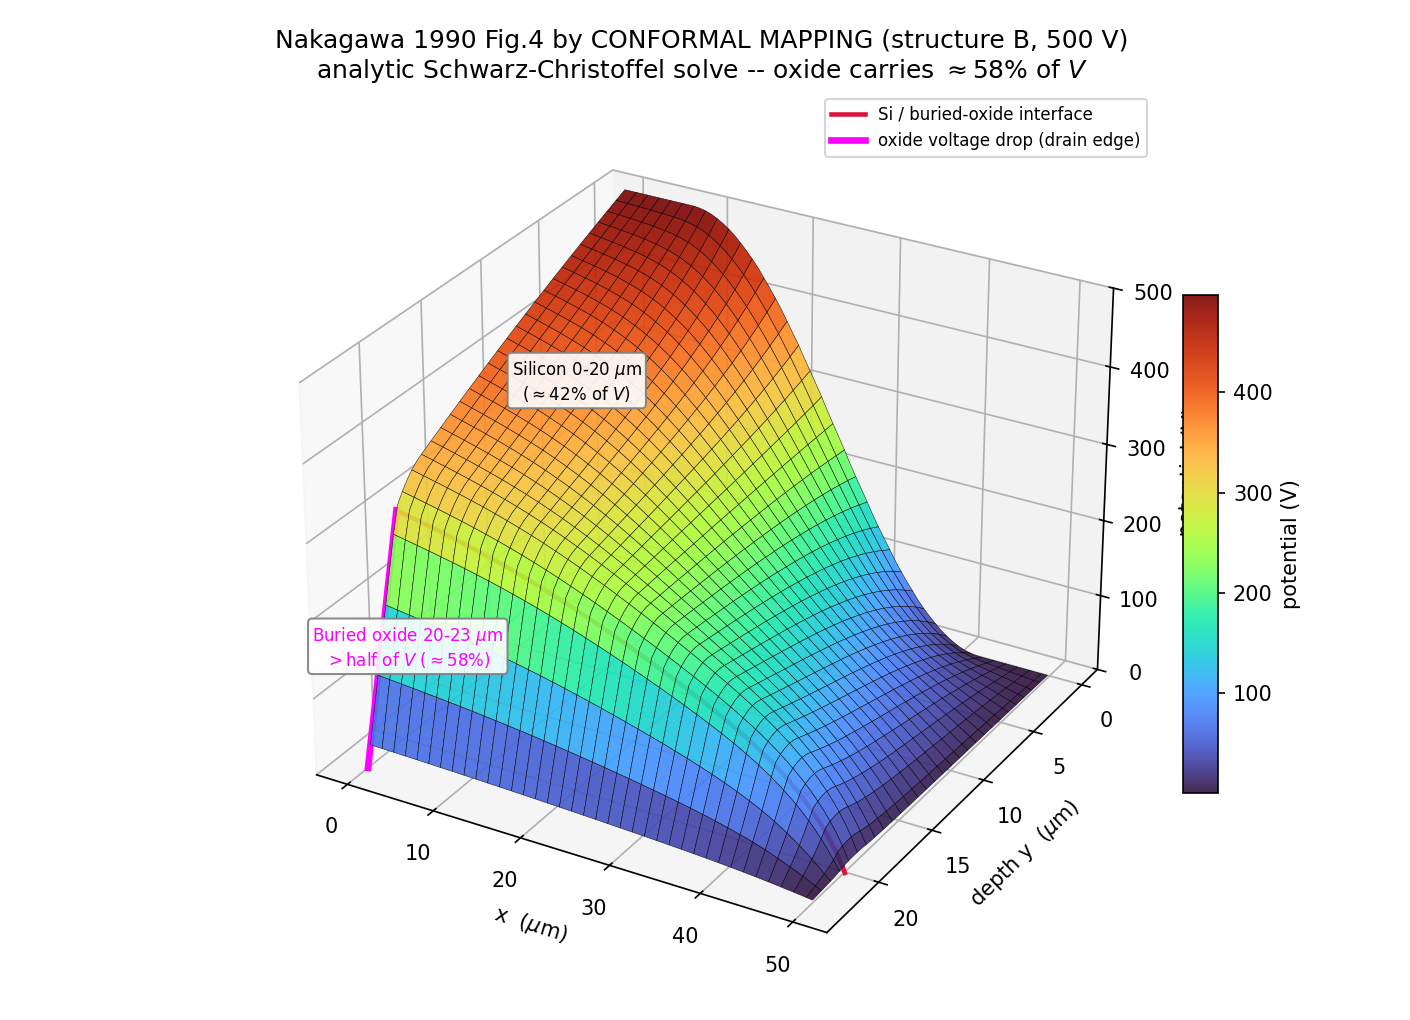
\includegraphics[width=\linewidth]{../figs/fig4_conformal_3d.png}
  \caption{Conformal map --- 3-D potential.}
\end{subfigure}\hfill
\begin{subfigure}{0.49\textwidth}\centering
  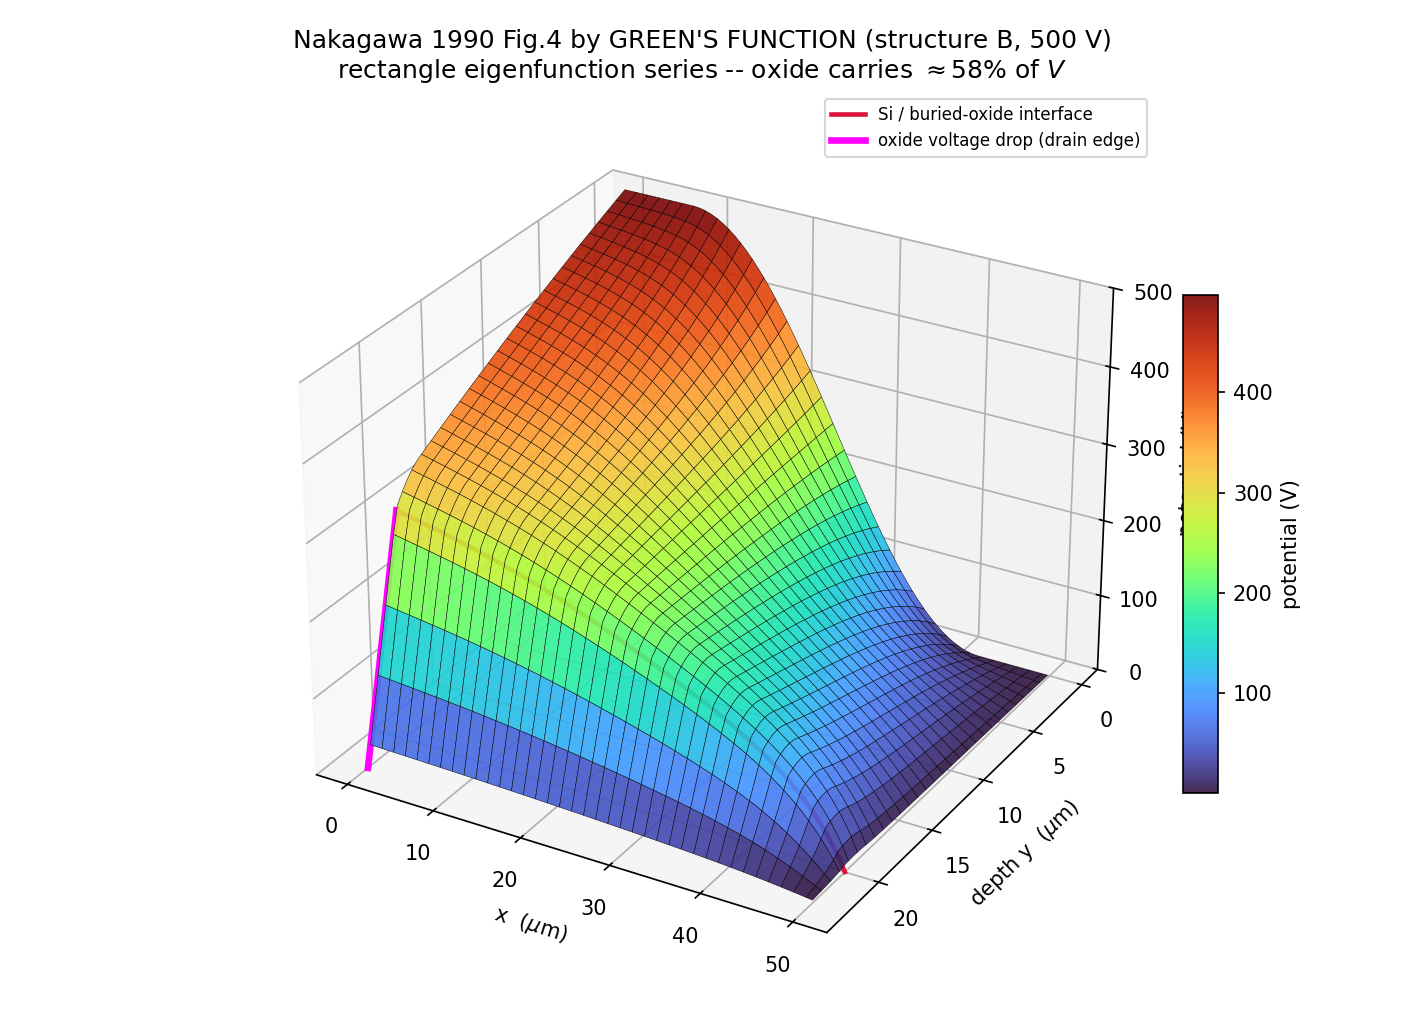
\includegraphics[width=\linewidth]{../figs/fig4_green_3d.png}
  \caption{Green's function --- 3-D potential.}
\end{subfigure}
\caption{The Fig.~4 potential surface from the two analytic methods. Both show the
gentle slope through the silicon and the steep ``voltage cliff'' across the buried
oxide at the drain edge (magenta), carrying $\approx58\%$ of $V$.}
\label{fig:3d}
\end{figure}

\begin{figure}[h]\centering
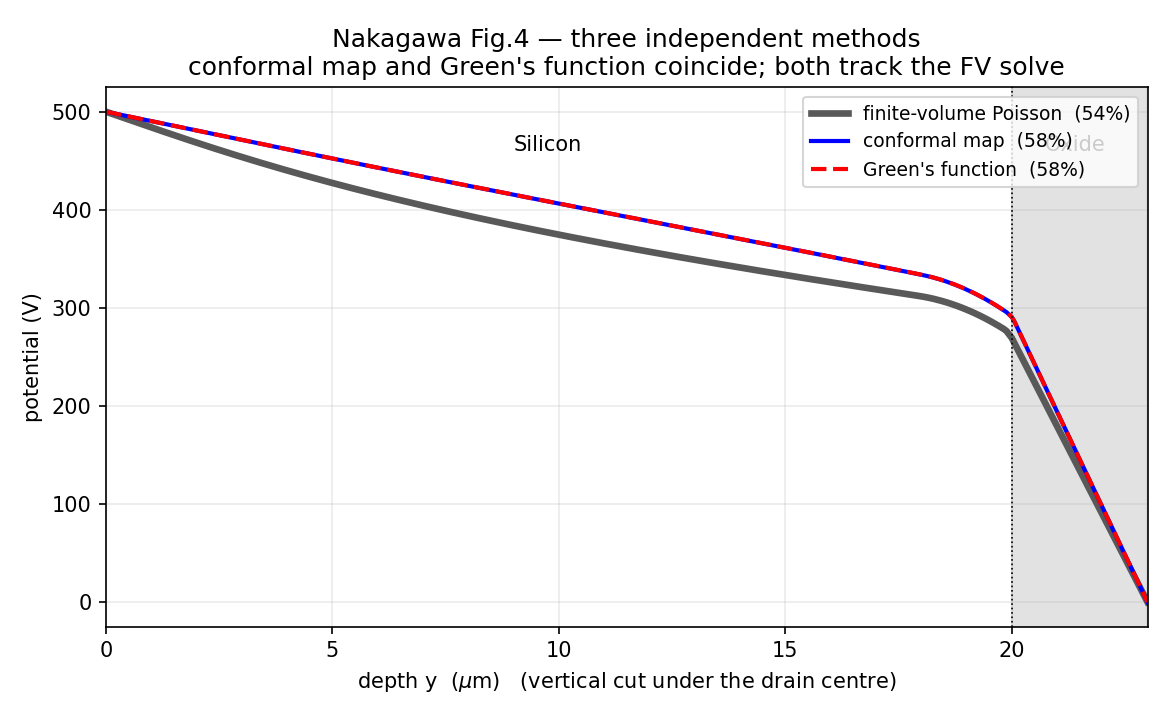
\includegraphics[width=0.74\textwidth]{../figs/fig4_three_methods.png}
\caption{Vertical cut under the drain centre for all three 2-D methods. The
conformal-map (blue) and Green's-function (red dashed) curves are visually
indistinguishable (RMS difference \SI{0.09}{\volt}); both track the finite-volume
Poisson solve (grey), differing only by the shared boundary-condition idealisation
in the silicon and converging across the oxide.}
\label{fig:three}
\end{figure}

\begin{table}[h]\centering\small
\caption{Oxide voltage share $s_{\mathrm{ox}}$ under the drain, and cross-checks.}
\begin{tabular}{@{}lcl@{}}
\toprule
Method & $s_{\mathrm{ox}}$ & note \\
\midrule
Finite-volume Poisson (Method 1) & $0.539$ & grid-converged $\approx0.54$; the yardstick\\
Conformal map (Method 2)         & $0.582$ & $\phih$ harmonic to $8\times10^{-16}$\\
Green's function (Method 3)      & $0.582$ & BCs exact; residual $\sim0.5\,V/\Heff^2$\\
\midrule
Charge-free divider              & $0.29$--$0.31$ & Laplace limit; dielectric ratio only\\
Paper (Fig.~4)                   & $>0.5$ & ``more than half''\\
\bottomrule
\end{tabular}
\label{tab:share}
\end{table}

\begin{figure}[h]\centering
\begin{subfigure}{0.49\textwidth}\centering
  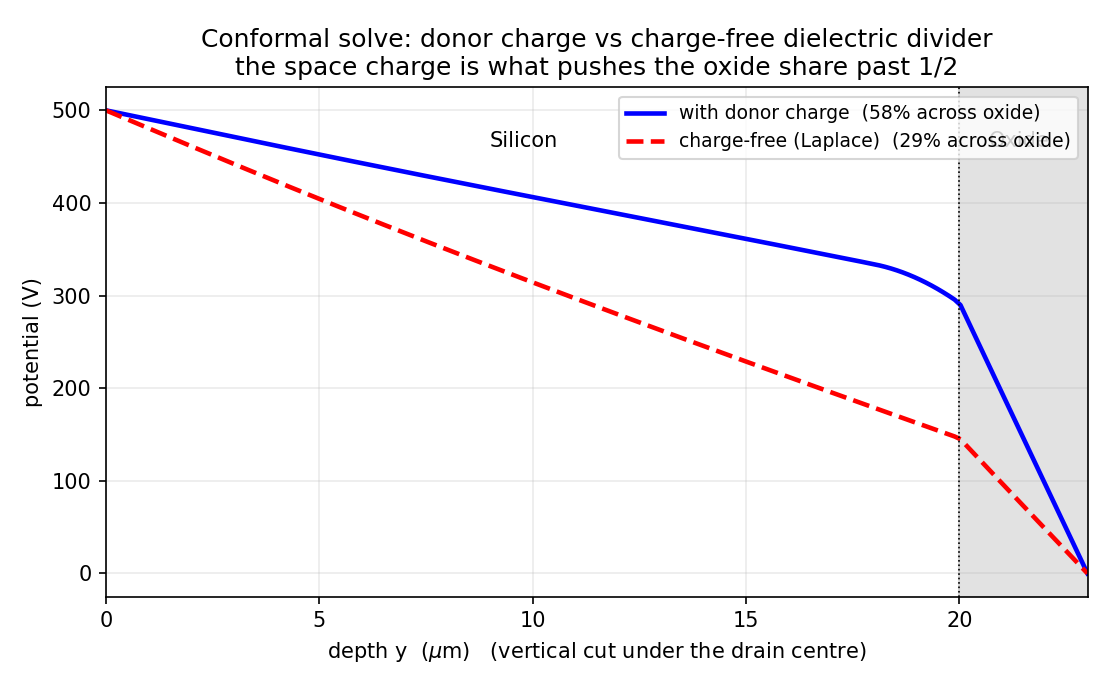
\includegraphics[width=\linewidth]{../figs/fig4_conformal_chargefree.png}
  \caption{Donor charge vs charge-free.}
\end{subfigure}\hfill
\begin{subfigure}{0.49\textwidth}\centering
  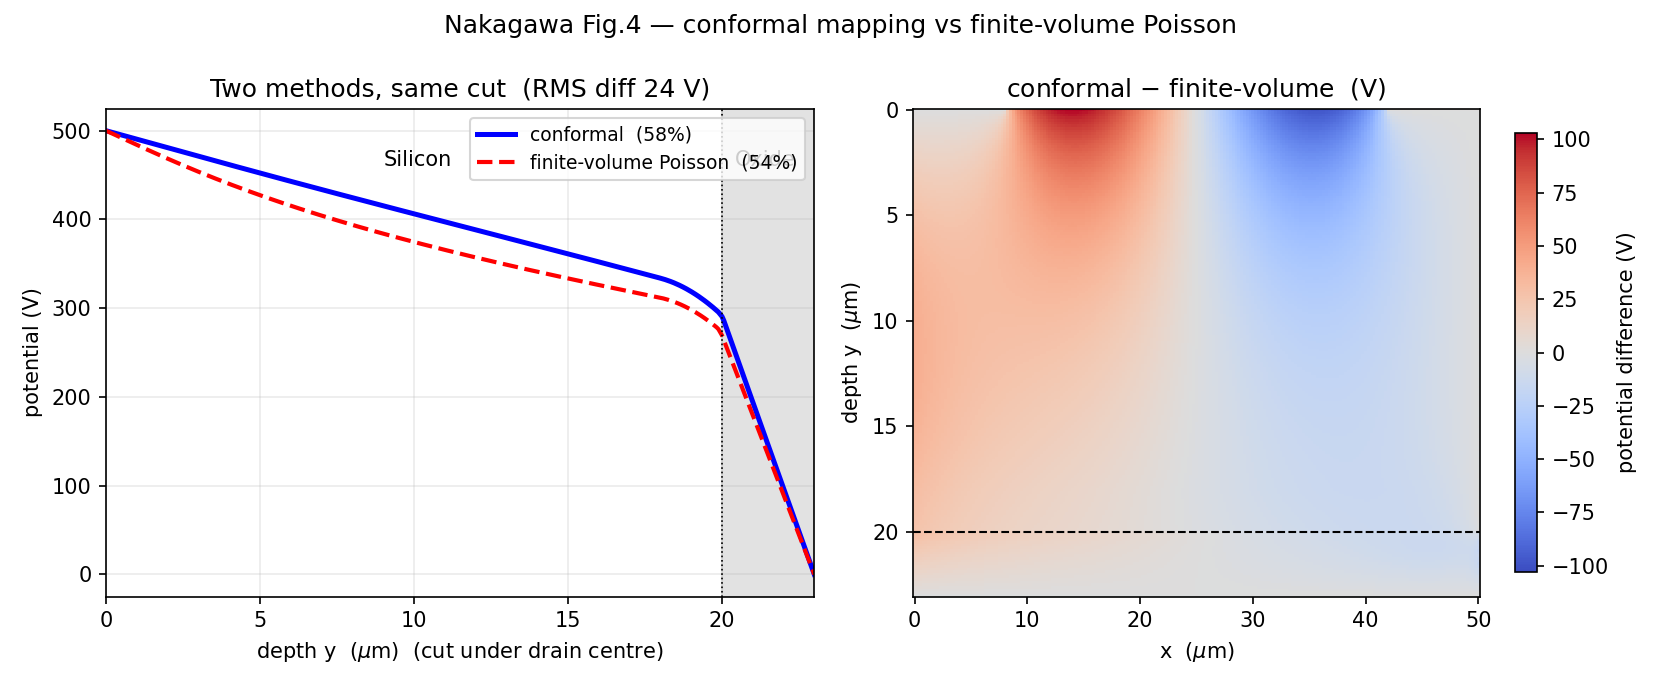
\includegraphics[width=\linewidth]{../figs/fig4_conformal_vs_fv.png}
  \caption{Conformal $-$ finite-volume difference.}
\end{subfigure}
\caption{(a)~Removing the space charge collapses the oxide share from $58\%$ to
$29\%$: the donor sheet, not the dielectric ratio alone, produces the ``more than
half'' result. (b)~The analytic$-$numeric difference is confined to near-surface
dipoles at the electrode edges (the BC idealisation); the bulk and the entire
oxide agree.}
\label{fig:diff}
\end{figure}

\subsection{Discussion}
Three observations close the loop:
\begin{itemize}\itemsep2pt
\item \textbf{The two analytic methods agree to \SI{0.09}{\volt} RMS.} The
conformal map (elliptic functions, harmonic measure) and the Green's function
(eigenfunction series) solve the \emph{identical} idealised boundary-value problem
by unrelated mathematics; their coincidence (Fig.~\ref{fig:three}) validates both
independently of the finite-volume solve.
\item \textbf{The residual $\sim5\%$ gap to finite volumes is the shared boundary
idealisation}, not a defect of either analytic method: it lives in near-surface
dipoles at the electrode edges (Fig.~\ref{fig:diff}b), exactly where the analytic
Dirichlet closures depart from the physical Neumann free surface.
\item \textbf{The space charge is the physics.} The charge-free divider gives only
$t_{\mathrm{ox}}/\eox \big/(\tsi/\esi+\tox/\eox)\approx0.31$; the donor sheet lifts
this by nearly $30$ points to $>\!\tfrac12$ (Fig.~\ref{fig:diff}a), reproducing the
paper's headline result.
\end{itemize}

% ==========================================================================
\section{Reproducing the figures}
% ==========================================================================
Each script is a standalone Python~3 entry point (numpy, scipy, matplotlib):
\begin{lstlisting}
cd nakagawa1990_repro/code
python fig4_pde_standalone.py   # Method 1: finite-volume Poisson  -> fig4_pde_standalone_3d.png
python fig4_conformal.py        # Method 2: conformal mapping      -> fig4_conformal*.png
python fig4_green.py            # Method 3: Green's function + 3-method compare
                                #           -> fig4_green*.png, fig4_three_methods.png
\end{lstlisting}
Numbers are printed next to the paper's values by each script's \texttt{verify()};
figures are written to \texttt{figs/}. Compile this report with
\texttt{pdflatex fig4\_multimethod\_report.tex} from \texttt{report/}.

\end{document}
